\chapter{Technické detaily}
Pro provoz webové aplikace je zapotřebí backend server.
Pro tento účel jsem zvolil ICT centrum VŠB-TUO, kde jsem si nechal
vytvořit virtuální server.

\section{Operační systém a konfigurace DNS}
Jako operační systém serveru jsem zvolil Rocky Linux,
který mi byl doporučen administrátory školní sítě. Tato linuxová
distribuce je založena na RHEL. Součástí konfigurace VM je také
nastavení sítě. Neměnná IP adresa je získána z DHCP serveru,
avšak se jedná pouze o IPv4. IPv6 je potřeba nastavit ručně.
Pro server je předkonfigurovaný také DNS záznam pro IPv4 a IPv6,
který vypadá následovně:

\begin{verbatim}
Name                       Type   TTL   Section    IPAddress
----                       ----   ---   -------    ---------
pol0423-stu.vsb.cz         AAAA   7200  Answer     2001:718:1001:207::64
pol0423-stu.vsb.cz         A      7200  Answer     158.196.109.64
\end{verbatim}

DNS záznam AAAA je vazba na IPv6 adresu, zatímco DNS záznam A
je vazba na IPv4.

\section{Instalace OS a počáteční konfigurace serveru}
Server se nachází na VMware vSphere serveru, dostupný
na adrese vcs.vsb.cz. Prvním krokem byla instalace OS Rocky Linux,
která proběhla přes virtuální konzoli serveru. Instalační program
byl ve formě GUI, přes které jsem nastavil uživatelský účet správce
\texttt{marpolda}, nastavil jsem mu heslo a zapnul mu práva správce.
Účet správce \texttt{root} je vypnutý, lze ho tedy použít jen pomocí
příkazu \texttt{sudo}. Po instalaci OS byla dalším krokem instalace
nástrojů virtuálního stroje. Po neúspěšném pokusu v instalaci balíčku
VMware Tools jsem se rozhodl využít místo toho otevřený balíček
\texttt{open-vm-tools}. Pro práci s textovými soubory jsem si
také nainstaloval balíček \texttt{nano}, který poskytuje jednoduchý
textový editor přímo v příkazovém řádku.

\begin{figure}
    \centering
    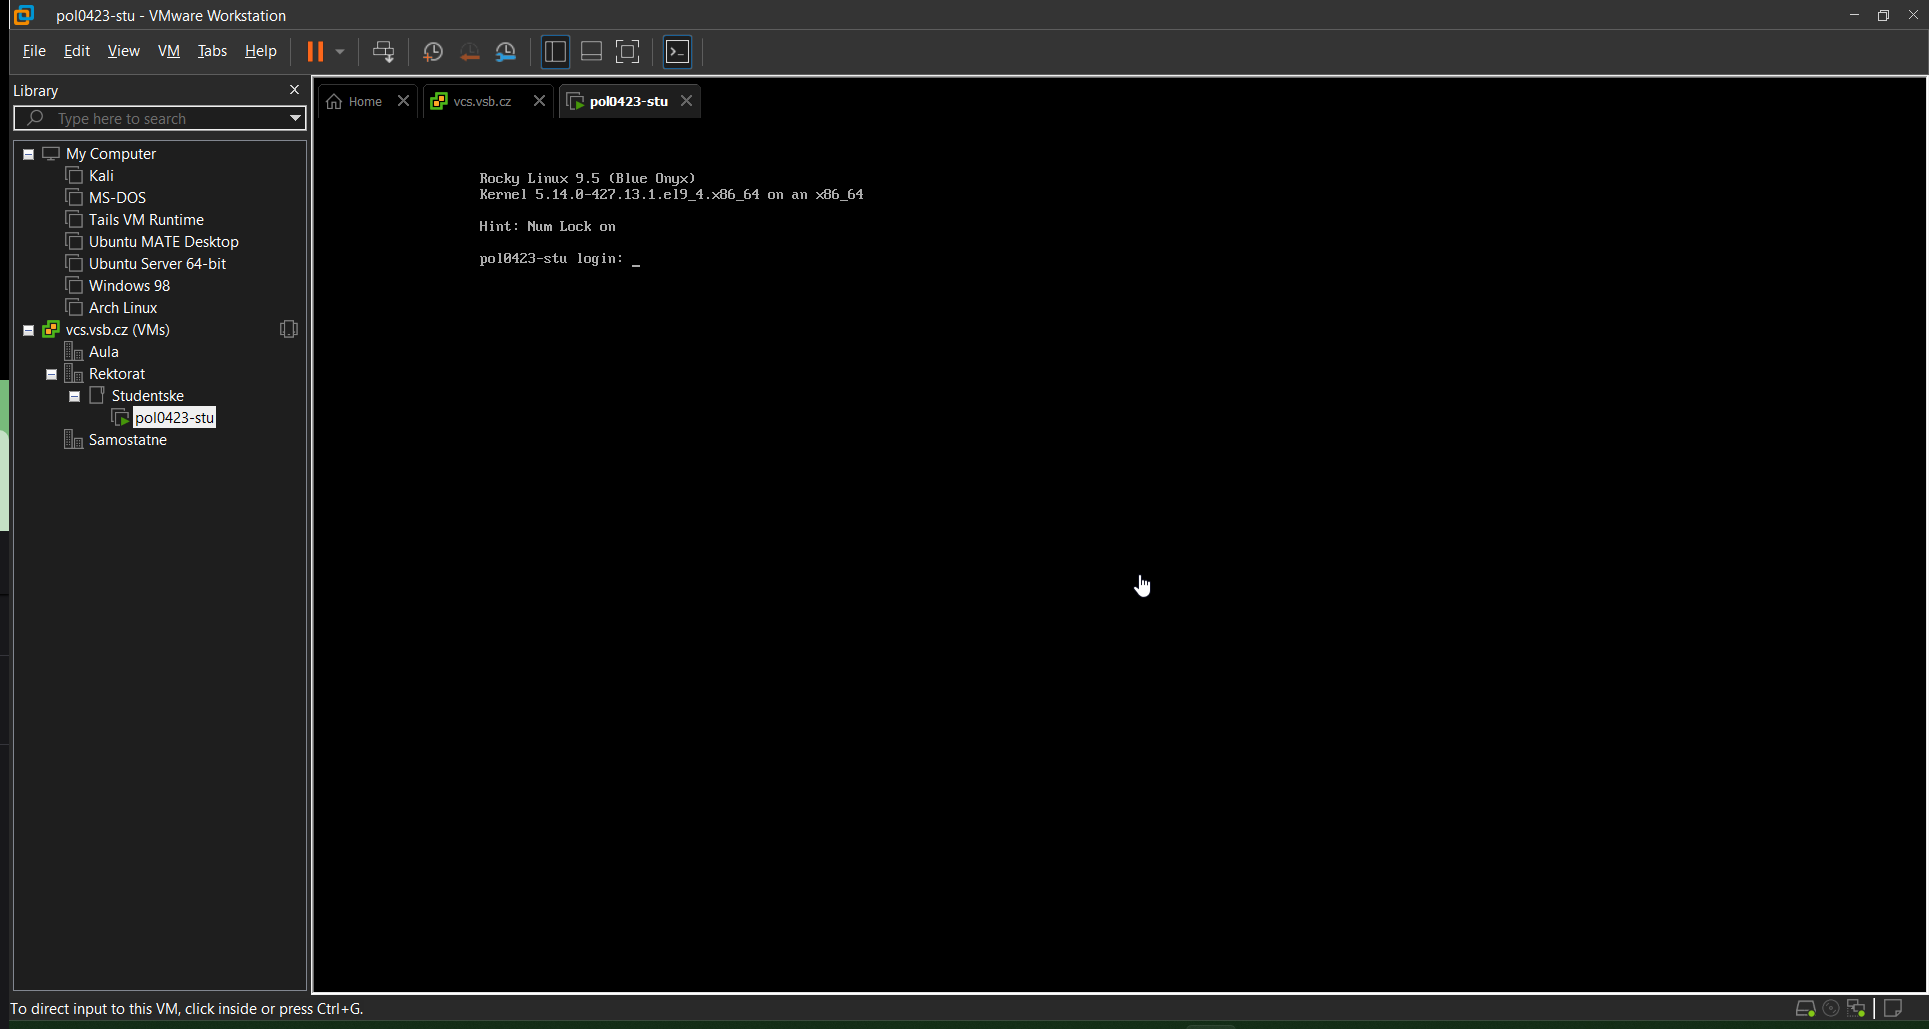
\includegraphics[width=0.75\linewidth]{Figures/vmware_console.png}
    \caption{Konzole virtuálního serveru ve VMware Workstation Pro}
    \label{fig:vmware-workstation-pro}
\end{figure}

Dalším krokem je nastavení IPv6 sítě. Jelikož IPv6 adresa není
DHCP serverem přidělena, je potřeba adresu nastavit ručně. Pro to
využijeme výše zmíněný DNS záznam pro IPv6 vazbu. Tento proces
je také zapotřebí provést pomocí virtuální konzole.

\begin{verbatim}
# ip -6 addr add 2001:718:1001:207::64/64 dev ens33
# ip -6 route add default via 2001:718:1001:207::1 dev ens33
\end{verbatim}

Pro přístup na server pomocí SSH jsem si také importoval ručně
přes konzoli SSH klíče obou mých počítačů, které využívají kvantově
rezistentní algoritmus \texttt{ed25519}. Z důvodu bezpečnosti jsem
také provedl vypnutí přihlašování pomocí uživatelského hesla.
Tento krok jsem provedl vytvořením nového souboru
\texttt{/etc/ssh/sshd\_config.d/01-nopasswordlogin.conf}
s následujícím obsahem:

\begin{verbatim}
#################################################
# Disable password logins
#################################################

PasswordAuthentication no
\end{verbatim}

Soubory v adresáři \texttt{/etc/ssh/sshd\_config.d} jsou automaticky
importovány v souboru\\
\texttt{/etc/ssh/sshd\_config}, který obsahuje konfiguraci SSH Daemon
serveru.

Následně stačilo restartovat službu SSH Daemon:

\begin{verbatim}
# systemctl restart sshd.service
\end{verbatim}

Přístup na server pomocí SSH jsem následně otestoval:
\begin{verbatim}
PS C:\Users\marpo> ssh marpolda@pol0423-stu.vsb.cz
The authenticity of host 'pol0423-stu.vsb.cz (158.196.109.64)' can't be established.
ED25519 key fingerprint is SHA256:oHy0UKZisrWxLKQtp5Xpezo53FNXZudKJ6/WVHeScI4.
This host key is known by the following other names/addresses:
    ~/.ssh/known_hosts:18: 158.196.109.64
Are you sure you want to continue connecting (yes/no/[fingerprint])? yes
Warning: Permanently added 'pol0423-stu.vsb.cz' (ED25519) to the list of known hosts.
Enter passphrase for key 'C:\Users\marpo/.ssh/id_ed25519':
Last login: Sat Mar  1 14:01:55 2025 from 158.196.52.150
[marpolda@pol0423-stu ~]$
\end{verbatim}

Z mého druhého počítače jsem se také úspěšně přihlásil:
\begin{verbatim}
[marpolda@archlinuxx-laptop ~]$ ssh pol0423-stu.vsb.cz
Enter passphrase for key '/home/marpolda/.ssh/id_ed25519':
Last login: Sun Mar  2 19:21:04 2025 from 2001:718:1001:698:99e2:f1ff:4e67:7618
[marpolda@pol0423-stu ~]$
\end{verbatim}

\section{Kontejnerizace a instalace služeb}
Nyní, když máme nastavený základní přístup, můžeme přistoupit
k instalaci softwaru pro kontejnerizaci a samotných kontejnerů
potřebných služeb. Pro kontejnerizaci jsem si vybral Docker,
který jsem nainstaloval z příslušného balíčku následovně:

\begin{verbatim}
# dnf install docker
\end{verbatim}

% TODO: Po dokončení konfigurace IPv6 nainstalovat kontejnery
%       pro jednotlivé služby (web crawler, databáze, apod.)

\endinput
